
\subsection{Parameterwahl des HOG3D}
Das Experiment von Scherer, Walter und Schreck in \cite{scherer2010histograms} hat gezeigt, dass die Parameterwahl für den HOG3D die Performance stark beeinflussen kann. Eine sich als optimal erwiesene Einstellung ist in \figurename~\ref{Parameter} zu finden.

\begin{table}[H]
	\centering
	\caption{Optimale Parameterwahl für HOG3D, entnommen aus \cite{scherer2010histograms}}
	\label{Parameter}
	\begin{tabular}{ll}
		Parameter                & Wert     \\
		r\textsubscript{x,y,z} & $\frac{2}{52}$    \\
		c\textsubscript{x,y,z} & 12 vxl   \\
		bins($ \theta $)       & 9        \\
		bins($ \phi $)         & 9        \\
		b\textsubscript{x,y,z} & 2 Zellen \\S
		o\textsubscript{x,y,z} & 0 Zellen \\
		Dimensionalität          & 5184    
	\end{tabular}
	
\end{table}
Der Parameter r\textsubscript{x,y,z} legt die Anzahl der Voxel im Distanz Feld fest. r\textsubscript{x,y,z} steht jeweils für die Kantenlänge jedes Voxels. Je kleiner die Kantenlänge gewählt wird desto weniger Informationen gehen verloren, jedoch erhöht sich die Rechenzeit. Die Zellengröße c\textsubscript{x,y,z} legt fest wie viele Gradienten in ein Histogramm aufgenommen werden. Damit lässt sich der Grad der Lokalität des Deskriptors festlegen \cite{scherer2010histograms}.
Mit den Parametern 	bins($ \theta $) und bins($ \phi $) wird die Feinheit der Einteilungen des Histogramms festgelegt. Hier hat man die Wahl zwischen Genauigkeit und Stabilität.
Die nächsten beiden Parameter legen jeweils die Größe der Blöcke (b\textsubscript{x,y,z})  und ihre Überlappung  (o\textsubscript{x,y,z}) fest. Damit wird festgelegt, wie viele Benachbarte Zellen miteinander normalisiert werden. Diese beiden Parameter wurden zunächst vielversprechenden Parametern aus \cite{dalal2005histograms} gewählt. Die Überlappung hatte jedoch nicht den erwarteten positiven Effekt. Deshalb wurd der Wert 0 gewählt.


\subsection{Alternative Gradientendefinition}
Durch Experimentieren hat sich herausgestellt, das sich die 2. Ableitung für die Gradientenberechnung des HOG3D als effektiver erwiesen hat. Scherer, Walter und Schreck \cite{scherer2010histograms} begründen es damit, dass nicht nur Informationen über Lokale Extrema in der nähe Oberfläche des Meshs, sondern auch Informationen innerhalb des Meshs nützlich sein können. 
 \begin{figure}[thpb]
 	\centering
 	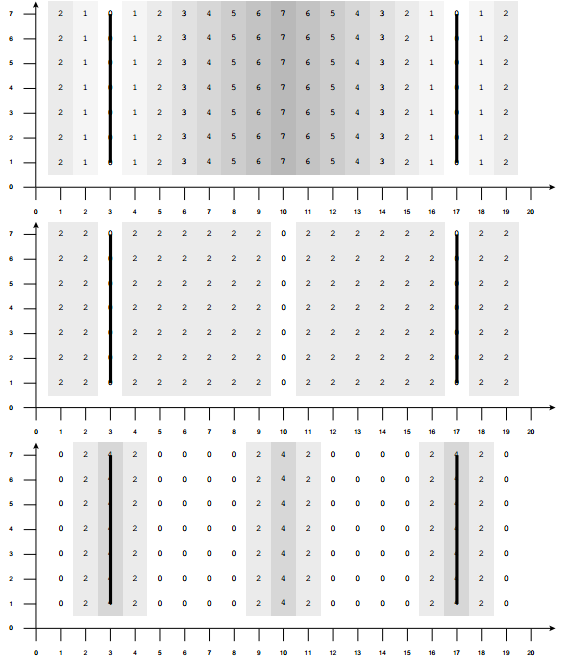
\includegraphics[width=\linewidth]{3-Diskussion/pics/2D_distance_field.png}
 	\caption{2D Darstellung eines Distanz Feldes, entnommen aus \cite{scherer2010histograms}. Das oberste Bild zeigt das Eigentliche Distanz Feld, das mittlere unter Verwendung der 1. Ableitung, das untere mit der 2. Ableitung}
 	\label{2D_distance_field}
 \end{figure}
 Zudem liefert die 1. Ableitung nicht genau das, was man unter Gradienten in der Bildverarbeitung versteht. Einen Pixel kann man als einen Punkt in der Welt verstehen, in dem Informationen über das reflektierte Licht gespeichert werden. Der entsprechende Gradient würde z.B. an Ecken von Wänden an stärke zunehmen. \figurename~\ref{2D_distance_field} zeigt deutlich, dass dies bei der 1. Ableitung nicht der Fall ist. Die 2. Ableitung hingegen erfüllt die Grundauffassung von Gradienten in der Bildverarbeitung.
 \newline
 
 